\documentclass[conference]{IEEEtran}
\IEEEoverridecommandlockouts
\usepackage{cite}
\usepackage{amsmath,amssymb,amsfonts}
\usepackage{algorithmic}
\usepackage{graphicx}
\usepackage{textcomp}
\usepackage{xcolor}
\def\BibTeX{{\rm B\kern-.05em{\sc i\kern-.025em b}\kern-.08em
    T\kern-.1667em\lower.7ex\hbox{E}\kern-.125emX}}
\begin{document}

\title{Procedural generation of levels for the angry birds videogame using
evolutionary computation\\
}

\author{\IEEEauthorblockN{ Jaime Salinas-Hernández}
\IEEEauthorblockA{\textit{Department of Graduate Studies} \\
\textit{Tijuana Institute of Technology}\\
Tijuana, México \\
salinas.jaime1217@gmail.com}
\and
\IEEEauthorblockN{ Mario Garcia-Valdez} \IEEEauthorblockA{\textit{Department of Graduate Studies} \\
\textit{Tijuana Institute of Technology}\\
Tijuana, México \\
mario@tectijuana.edu.mx}
\and
\IEEEauthorblockN{ JJ Merelo} \IEEEauthorblockA{\textit{Department of Graduate Studies} \\
\textit{Universidad de Granada}\\
Granada, Spain\\
jmerelo@ugr.es}}

\maketitle


\begin{abstract}
In this paper, we propose an evolutionary algorithm that follows an open-ended
evolution approach to generate levels for the Angry Birds video game. The levels
themselves are composed of a set of birds that the player can throw with a
slingshot, a certain amount of pigs that they must destroy, and a given number
of pieces that conform structures that may or may not protect the pigs from
birds thrown at them. The current goal is the generation of diverse structures
that are playable in the game, having the additional characteristics of being
fun and enjoyable. We propose a multi-layered search, first constructing
composite structures from basic blocks, to then build more complex structures
building from these composites. We follow an open-ended evolution approach in
which the evolution of structures is not guided towards a single objective but
is rather free to evolve and generate novelty or diversity. The fitness function
we use to evaluate the proposed levels considers how complex levels have become
and how different they are from the rest of the population. The experiments
conducted show that an evolutionary approach allows the generation of levels
that are novel and interesting to play.
% Another revision to English would be good.
% Done - Mario
\end{abstract}

\begin{IEEEkeywords}
Genetic algorithm, procedural generated content, open-ended evolution,
evolutionary computation
\end{IEEEkeywords}
    
\section{Introduction}
The video game industry is always looking for content creators to satisfy
the demand for high-quality content. Current development teams include game
designers,  artists, animators,  writers, level designers, among others.
Procedural Content Generation (PCG) is often applied to generate many
aspects of the game, from maps, levels or characters, to narrative and game
design. PCG techniques can lower the cost in both time and human resources
when generating content for different video game projects, without
compromising qualitiy \cite{Yannakakis2017,YannakakisContentGeneration}. In
this paper, we introduce an evolutionary content generation system, to
generate fun and exciting levels for the popular Angry Birds video game. We
follow an Open-Ended Evolution (OEE) approach.  OOE is a type of genetic
evolution algorithm with a different objective. In this case, the goal is
not to reach a final state of in the evolution, for instance, to reach an
optimal solution in a search space. An OEE aims to continue evolving and
creating new types of entities, perhaps more complex or novel on each new
generation. Entities evolve not only inside the frame of their species, but
they can also create entirely new species \cite{Standish2003}. Taylor et al.
\cite{Taylor2016, Taylor} define OEE as a system capable of creating novelty
beyond a point where nothing changes on the current group of interest rather
than just converging to a stable or quasi-stable state. For this project,
OEE is defined simply as a genetic algorithm with different classes of
objects, with compositional and taxonomic relationships between them.
Objects in a class can evolve in parallel or as in this case, independently
of each other. The object-oriented model follows these principles to model
complex behavior and structure \cite{levesque1986knowledge}. 

The case study for this paper is to follow the rules of a level generation
competition for the Angry Birds video game developed by Rovio Entertainment.
We briefly explain the game.  The objective is to destroy structures placed
on a map as well as eliminating green pig-like characters. In order to
obtain the highest score possible, the game uses a gravity and collision
system that allows the structures to fall and be destroyed by means of
damage. The structures have  three different construction materials
\textit{ice}, \textit{wood} and \textit{stone}, each one with a different
resistance, ranging from fragile, normal and sturdy in that order. The game
mechanic is to use a slingshot to shoot a certain number of birds with
different abilities, to destroy both the structures and the objectives. A
high score is achieved by causing the most destruction throwing the least
birds possible \cite{RovioEntertainmentCorporation2009}. The main objective
of this work is to generate levels that can be played by naïve or
intelligent agents as well as human players. The levels themselves need to
be complex in the sense that interesting structures can be created, but at
the same time, remaining possible to complete in some way \cite{Stephenson,
Stephenson2018}.
% What is the problem?

One peculiarity of PCG is the richness of problems and domains in which it can
be applied.  This is because each type of game dictates different restrictions
and mechanics. In this case, we have additional restrictions, dictated by the
competition track \cite{Renz}. This case study provides an interesting challenge
for the participating algorithms. The proposed PCG algorithm has to be flexible
on the pieces it can use, and also consider the running time, as both are
determined at runtime. The aim is to develop a software capable of creating game
levels having the objective of being both \textit{interesting} and
\textit{playable}. Candidate solutions, in this case, Levels of the game, will
be evaluated by using the open-source software Science Birds \cite{sciencebirds}
which uses the same resources used on the original angry birds game. Using this
software for the evaluation is an additional restriction because we are limited
to the data collected during the simulation.  
% What is learned?
In this work, we found that an evolutionary algorithm can be used to create this
type of content, because it is not only able to create levels that are
interesting and diverse but also capable of producing levels an average human
could have trouble imagining. The rest of the paper is as follows. Section
\ref{SoA}, contains a quick overview of some aspects used by different authors
to tackle this problem, their design, and basic functionality. In Section
\ref{prop_method} we describe our current proposal.  How we modeled the
candidate solutions and the way we defined our fitness function to determine the
playability and complexity of the generated levels. Finally, in Section
\ref{conclusion}, we provide our conclusions as well as improvements that can
help to refine the proposed work. 

\section{State of the art}
\label{SoA}
In this Section, we present PCG works relevant to the level generation for
the Angry Birds video game. Renz et al. \cite{Renz, Renz2015TheAB} organized
an AI competition to develop intelligent agents that could play new  Angry
Birds levels better than the best human players. The competition was then
collocated in other AI conferences. To better train and test agents, more
novel and some times, challenging levels must be generated. Stephenson et
al. proposed a related competition this time with the goal of developing a
level generator for the game. Researchers have proposed several generators
in the following years of competition. M. Katina et al.  \cite{Kaidan2015}
propose a model in which the algorithm controls the generation of content by
using the skill of a player, while she is actively playing the game. The
moment the player finishes a certain level, the algorithm obtains the score
and generates the next level to play. Y. Jiang et al. \cite{Jiang2017}
proposed the use of predefined letter patterns and combined them to create a
small pool of words and letters used to create levels with text on them.
Users would play the game, and after that,   asked them if they liked the
layout of the Levels.  Several researchers follow a search-based approach.
Calle et al. \cite{lauracalle} propose a free-search method to generate
levels.  For this, lists of blocks are placed in the game by the algorithm,
and those maintaining their positions against gravity are selected to build
structures. The resulting structures continue evolving into more complex
levels. That work is the basis of our current proposal, and since we are
using a modified version of the Angry Birds game, that can obtain data of a
level after a simulation.
    
    \section{Proposed Method}
    \label{prop_method}  

In this Section, we describe the approach used in this work, explaining
first, the restrictions of the game, then giving a quick overview of how we
create new composites to be used by the algorithm, then we define how candidate
solutions are to be represented by the algorithm. We then describe our method to
evaluate candidate solutions. Finally, we present details of the evolutionary
algorithm. 

The game contains a total of 11 block shapes, shown in Figure
\ref{piece_list}. These basic blocks cannot be modified, and we can not add
more. With this in mind, we propose to create additional elements by creating
composites of these blocks. Atomic blocks can be positioned in different
locations and at certain angles, inside the composite. The resulting composites
are themselves the new building blocks of more complex structures. 
    
\subsection{Composite Generation}

Since there is no way to \textit{add} a new composite to the pool of blocks, we
first need a way to combine them. To do this, first, the original 11 blocks of
the game need to be converted into composites of a single element.  We define a
composite as a list of blocks; then  \textit{composite} with a single block,
will be created for each original block. Composites are the first layer, the
building blocks for the structures to come. A composite could include different
types of blocks, rotated at a certain angle and compose a basic structure. An
ideal composite could support other composites on top without falling apart, but
this is not required. A composite is measured using an imaginary bounding box,
defined by calculating the lengths of all the pieces, finding the borders of
said pieces and then finding the points to define a box around all of them. We
then use this defined box to calculate the height and width of the new
composite. Then we derive from the center point of the said box, the offsets for
each block in the composite, as shown in figure \ref{bounding_boc_calc}. We need
this information to treat each composite as if it was a single block; this will
enable the placements of the composites in their respective new position when we
create the files needed for the simulation. This process is similar to creating
a group of elements in a drawing application.

    %% 
Suitable composites can be found using an evolutionary approach proposed
earlier by Calle and Merelo, where basic structures are generated by freely
searching a space of falling blocks and selecting those that remain
standing. This algorithm is not capable of creating complex structures, but
it can produce original basic structures. We can see that evolution at this
level can benefit from having more freedom when building basic structures.
At this time, we do not want to form piles or sequences of blocks, this will
be done later, at a higher level in the composite hierarchy.    
At this level the composite generator has the following steps:
\begin{enumerate}
\item Generate the first generation of the population, consisting of
randomly generated list of blocks.
\item Run a Simulation.
\item Evaluate each individual of the population.
\item If a member of the population has remaining pieces obtain the location
and angle of the pieces, assign a fitness.
\item Do the selection, crossover and mutation operations.
\item Repeat the cycle.
\item From the best individuals select composites. Several algorithms could
be proposed for this step, for instance selecting clusters of blocks.
\end{enumerate}
    
Another valid option is to generate interesting composites manually.  The
algorithm can later use the composites. We could say that the approach we
explained earlier, is an optional procedural generation of composites.

\begin{figure}[htbp]
\centerline{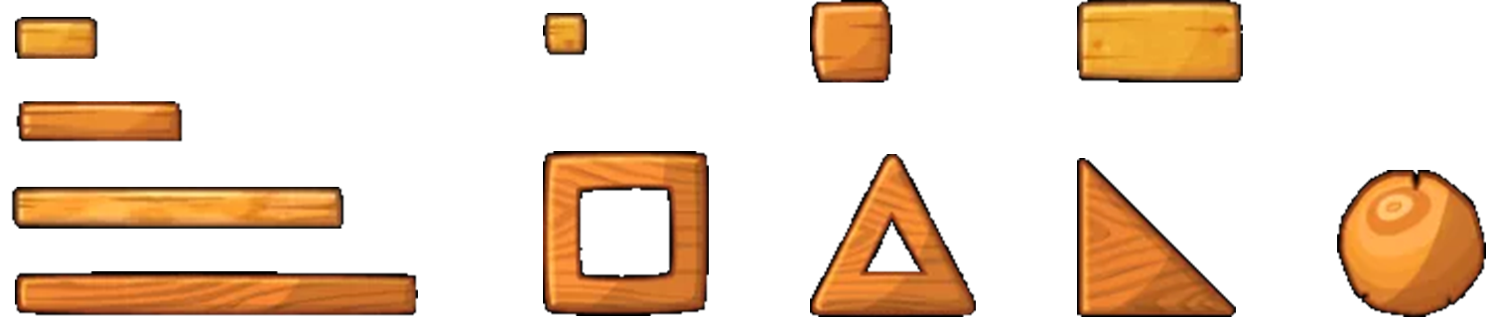
\includegraphics[width=80mm]{Images/list_pieces.png}}
\caption{List of blocks in the angry birds game.}
\label{piece_list}
\end{figure}

The Angry Birds level generation track is a competition where the objective is
to generate levels that are \textit{fun} and \textit{enjoyable}; they also have
to be challenging but not impossible. The rules for the competition specify that
a configuration file must be used to generate the levels of the game in a
limited amount of time. The file contains several restrictions;
namely:\begin{itemize}
\item   The number of \textit{different}
levels that must be generated. 
\item The materials that are \textit{not allowed}.

For instance, a group of generated levels must not have spheres composed of  is
ice or stone. Moreover, a banned material can not integrate others. 
\item The third configuration value is the \textit{number of pigs} that we must
place in a level. 
\item Finally, the \textit{limit} of time that the system has to generate the
required amount of levels.
\end{itemize}

We will present next a system for evolving structures that respects those restrictions.

\subsection{Structure Evolution}
   
    \begin{figure}[htbp]
    \centerline{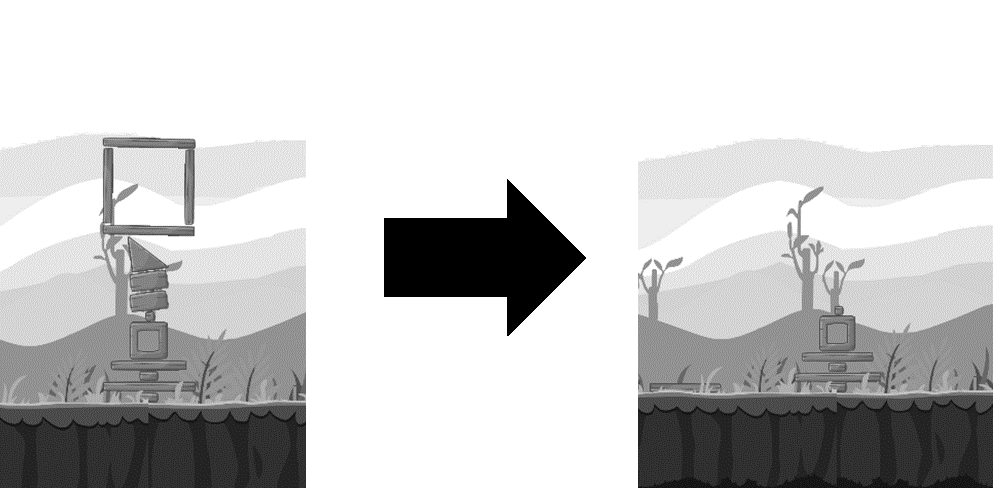
\includegraphics[width=80mm]{Images/simulation_bef_aft_example.png}}
    \caption{Structure at the beginning and end of a simulation.}
    \label{test_old}
    \end{figure}
    %
Structures are the next evolutionary layer, at a higher level of composition.
Structures are compositions of composites. A level can be seen as a collection 
of structures and each structure is a pile of composite blocks. This way of 
constructing levels has the advantage of
limiting the search space to structures that have a better chance to be 
standing after the simulation ends. There is no warranty that piles of 
composite blocks will keep the balance, so again we must search for those 
structures.

Structures are represented in a way similar to Togelius et al.
\cite{togelius2016Representationsforsearch-basedmethods}. We can model a
structure as a collection of composites, each one selected from a pool of
currently available composites. Initially, the pool contains only the 11
original blocks represented as single-element composites. As new composites are
automatically (or manually) generated from the original blocks, we insert them
to the pool and assign each one an ID. We can model the chromosome of a
structure, as shown in Figure \ref{old_chrom} where each gen is an ID from a
composite in the pool. A chromosome can include the same ID multiple times.
    % I don't understand this too well, maybe rephrasing would clarify - JJ
    % Done - Mario
    
    \begin{figure}[htbp]
    \centerline{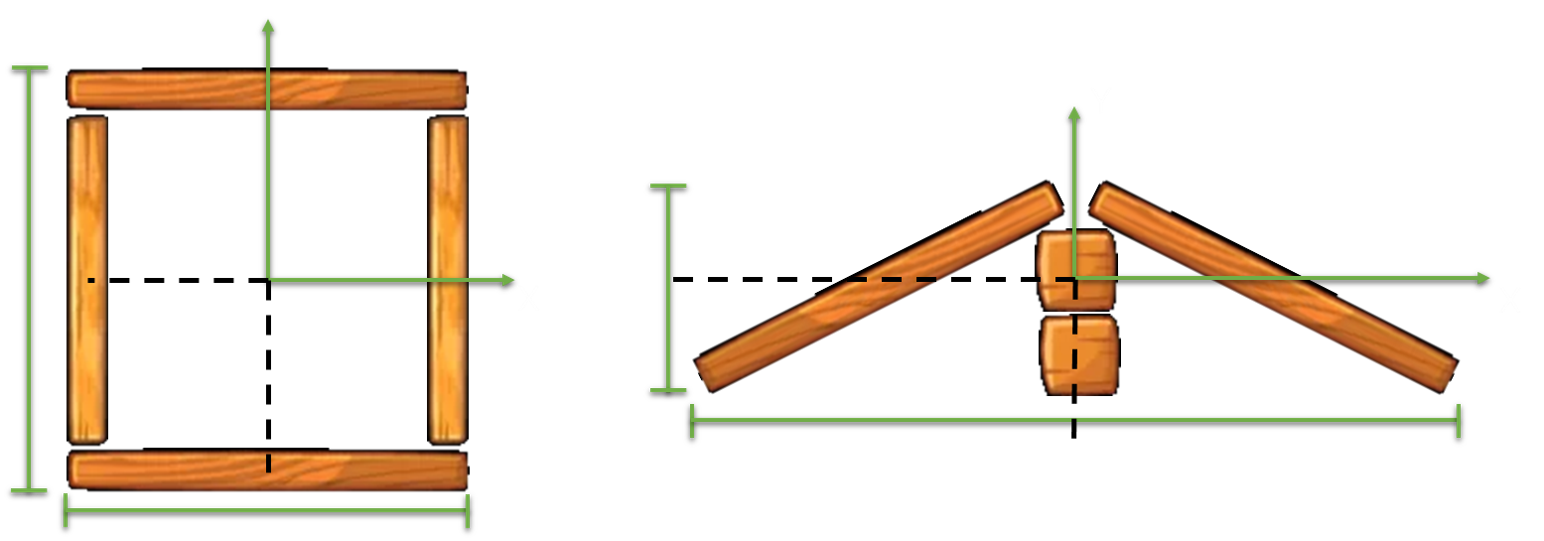
\includegraphics[width=80mm]{Images/bounding_box_calculation.png}}
    \caption{Bounding box calculation.}
    \label{bounding_boc_calc}
    \end{figure}
    
    \begin{figure}[htbp]
    \centerline{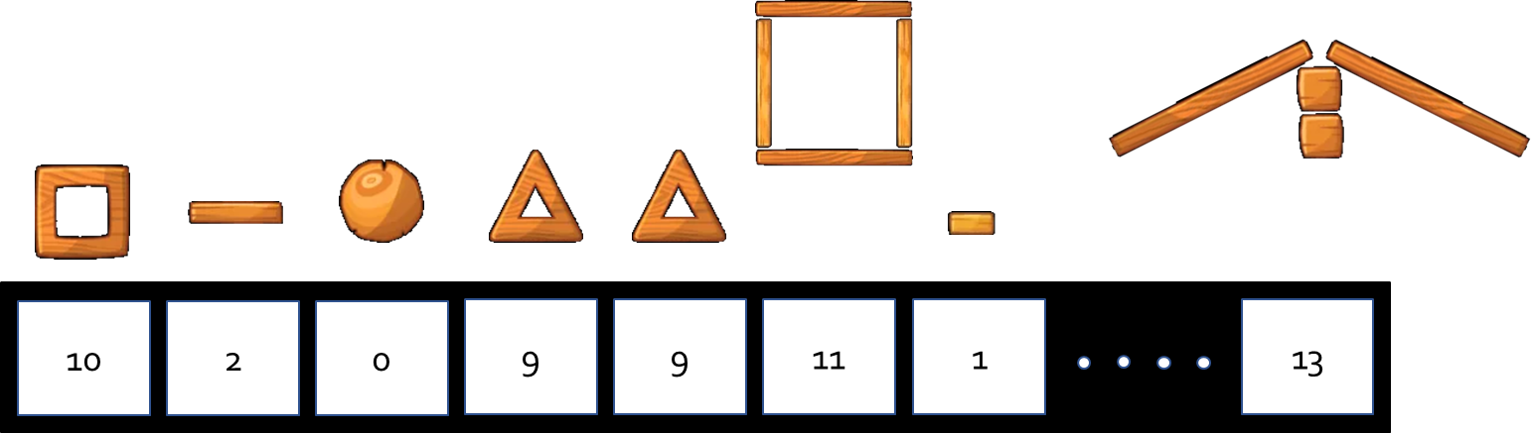
\includegraphics[width=80mm]{Images/chromosome_chain_example.png}}
    \caption{Chromosome chain of an individual.}
    \label{old_chrom}
    \end{figure}
    
    These structures represent individuals in the evolutionary algorithm. Once
    an individual is created it is ready to be evaluated in a simulation on the
    game environment. %In Laura's work, we tried to avoid this because it took a long time. Is there any procedure to check constraints and not evaluate them? - JJ
    % I will comment that we could work on that. At the moment each one is evaluated. - M 

    Using a similar approach as the composite generator, all
    individuals have a maximum of ten seconds to maintain balance or reach
    absolute stability. If that happens  it means one of two
    things, first the generated structure is completely stable or second, the
    tower fell to either side and the pieces were destroyed or stopped moving by
    gravitational pull, when either of this happens by more than two seconds the
    simulation ends regardless of time remaining and the next individual is
    simulated.

    The evaluation process for this project is still in the development stages,
    and in our experience is one one of the more difficult components in this
    kind of systems. In this stage of the evolution, we first need to assign a
    good fitness to those structures that keep their balance and not fall apart.
    There are other variables we take in to account, but they will be explained
    later. In this initial stage, each individual in the population has 100
    points so before the simulation starts each of them are viable candidates to
    be an Elite % Elite? - JJ
    % But I think the problem remains, there is no difference even if they all have
    % zero points. But randomess in the selection coyuld do that. - Mario
    member of the population regardless of their relative height or
    complexity.
    
    First, after each of the individual simulations are over the evaluation process
    takes place, in this phase the resulting level is checked for those blocks that
    survived, that is,  not destroyed by falling. Every one
    of them is counted and then the resulting number is compared to the
    initial quantity of pieces  before the simulation. Each block represents a certain percentage of 100\% so the missing pieces 
    are subtracted from the total. In this moment, each block is counted as if 
    it was not a member of a composite, this is because after the simulation there is
    only data about each individual block. % What is a composite? The fitness is only the number of remaining blocks? Even if they are in the floor?
    

    \subsection{Structure Positioning}

     The positioning of structures in the map is important in order to generate
     levels that are fun and aesthetically pleasing. For this we need a method to indicate the
     positioning of each structure. We propose the use of a mask where the
     positioning of each pile and the number of blocks it contains is specified.
     Again these masks could be manually created, for instance using the rule of
     thirds \cite{DarrenRowse} which is a guideline used while creating images,
     the purpose is to create aesthetic pleasant images where the focus point
     or the most important area is at the center of the image as shown on figure
     \ref{rule_of_thirds}, using this rule different distribution groups or
     masks are created has shown on figure \ref{rule_of_thirds_masks} in order
     to use them before the simulation of an individual by placing the pieces in
     order to distribute them in a way that can cover more area and create more
     balanced levels instead of using a tower like distribution as shown on
     figure \ref{results_old}. There is an option in the system to generate in a
     first step a collection of masks, following these rules, but this approach
     % in many cases this is used instead of these. Please check that - JJ
     has a drawback. Pre-generating masks would not allow the generator to
     \textit{evolve} because the individuals would be limited to a certain
     number of possibles combinations which will in turn prevent diversity in
     the population, so in order to prevent this we proposed an approach that
     allows the individuals to generate a mask in which a number of columns is
     defined by default but the amount of pieces in each one is random, however
     the total amount of assigned blocks in all columns must be the same as the
     total pieces allowed in each individual. The number of maximum blocks is
     a parameter. An example of this can be seen in figure \ref{new_chrom} where
     the total of pieces in a individual is 18 and these pieces are distributed
     on all the columns available.

     \begin{figure}[htbp]
        \centerline{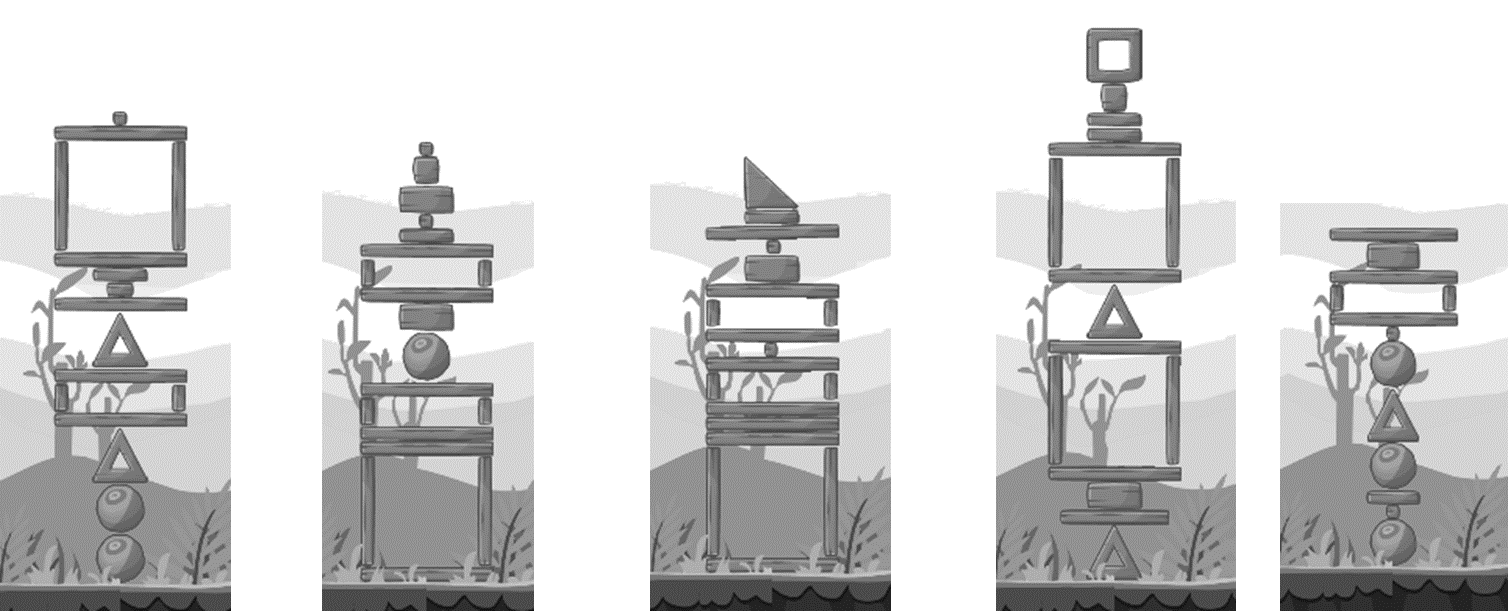
\includegraphics[width=80mm]{Images/result_example.png}}
        \caption{Result samples of current system.}
        \label{results_old}
    \end{figure}
    %
    \begin{figure}[htbp]
        \centerline{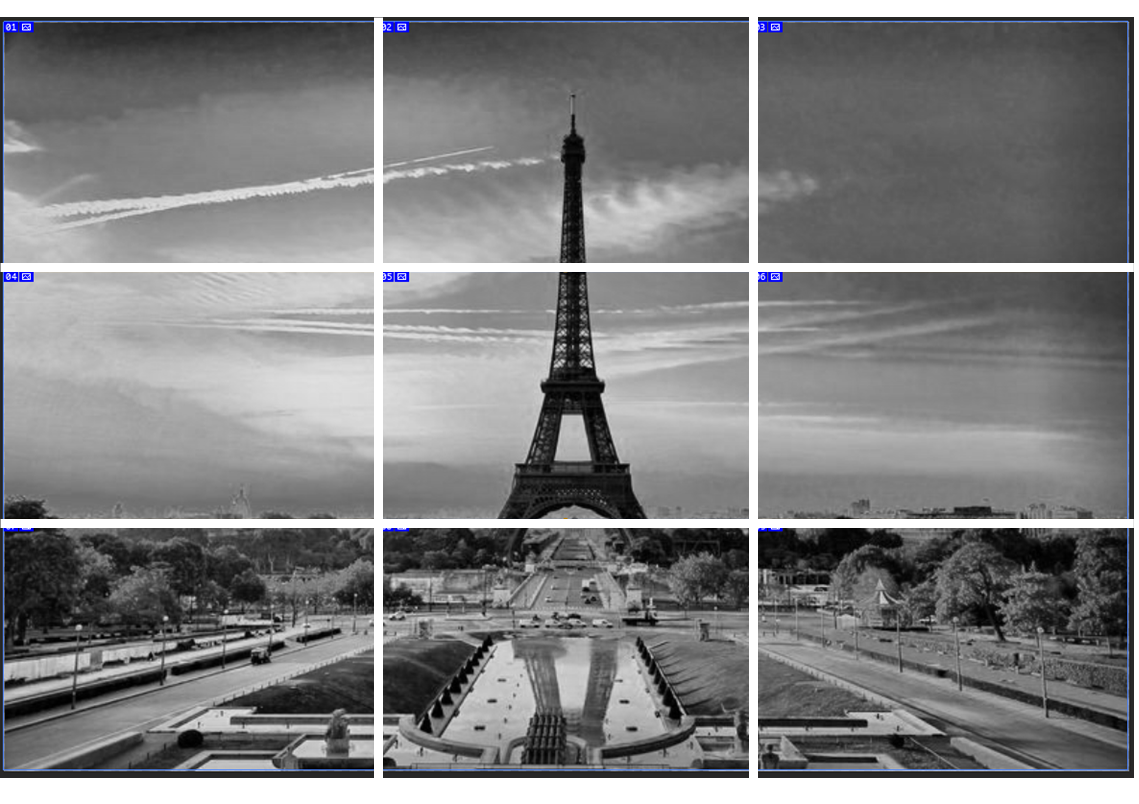
\includegraphics[width=80mm]{Images/ruleofthirds_example.png}}
        \caption{Rule of thirds example.}
        \label{rule_of_thirds}
    \end{figure}
    %
    \begin{figure}[htbp]
        \centerline{
\includegraphics[width=80mm]{Images/mask_distribution.png}}
        \caption{Masks created using the rule of thirds.}
        \label{rule_of_thirds_masks}
    \end{figure}
    %
    %
    \begin{figure}[htbp]
        \centerline{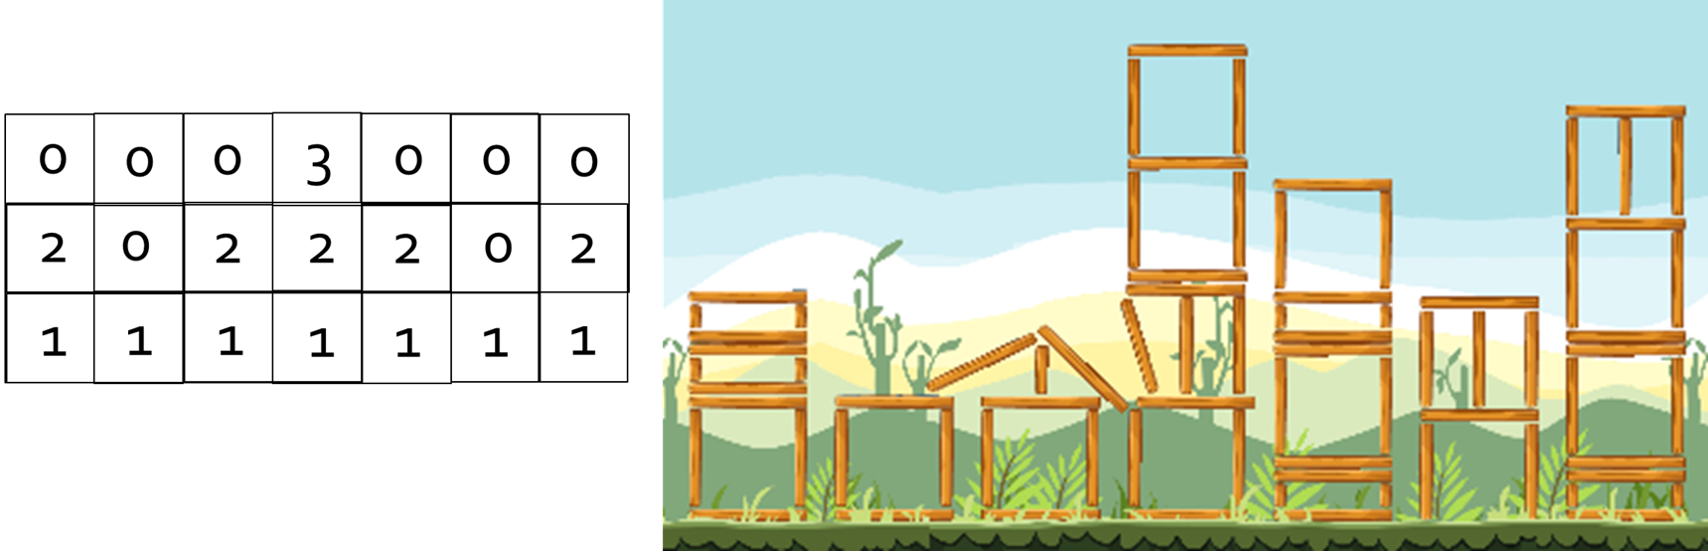
\includegraphics[width=80mm]{Images/result_example_thirds.png}}
        \caption{Results obtained with rule of thirds.}
        \label{rule_of_thirds_result}
    \end{figure}
    %
    \begin{figure}[htbp]
    \centerline{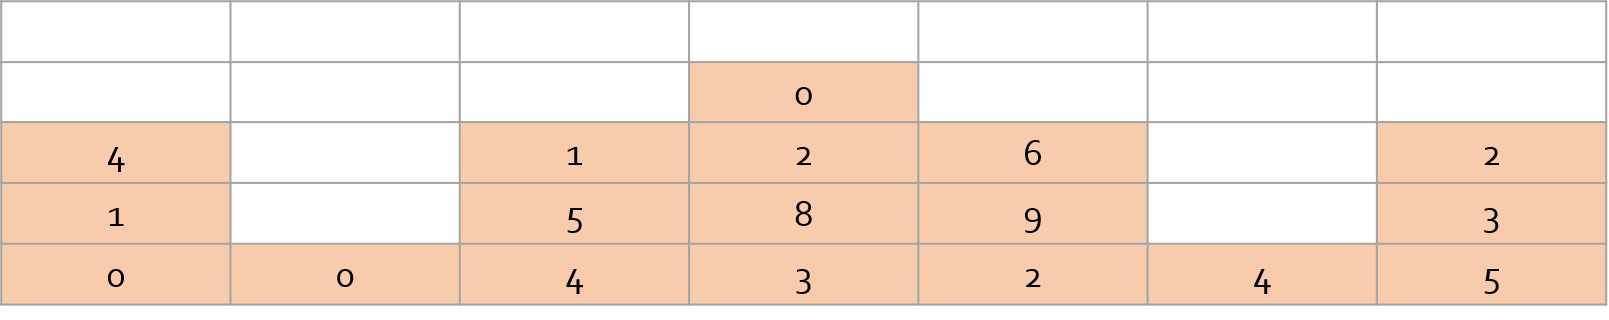
\includegraphics[width=80mm]{Images/chromosome_chain_new_model.png}}
    \caption{New chromosome chain.}
    \label{new_chrom}
    \end{figure}
    %
    \begin{figure*}[htbp]
    \centerline{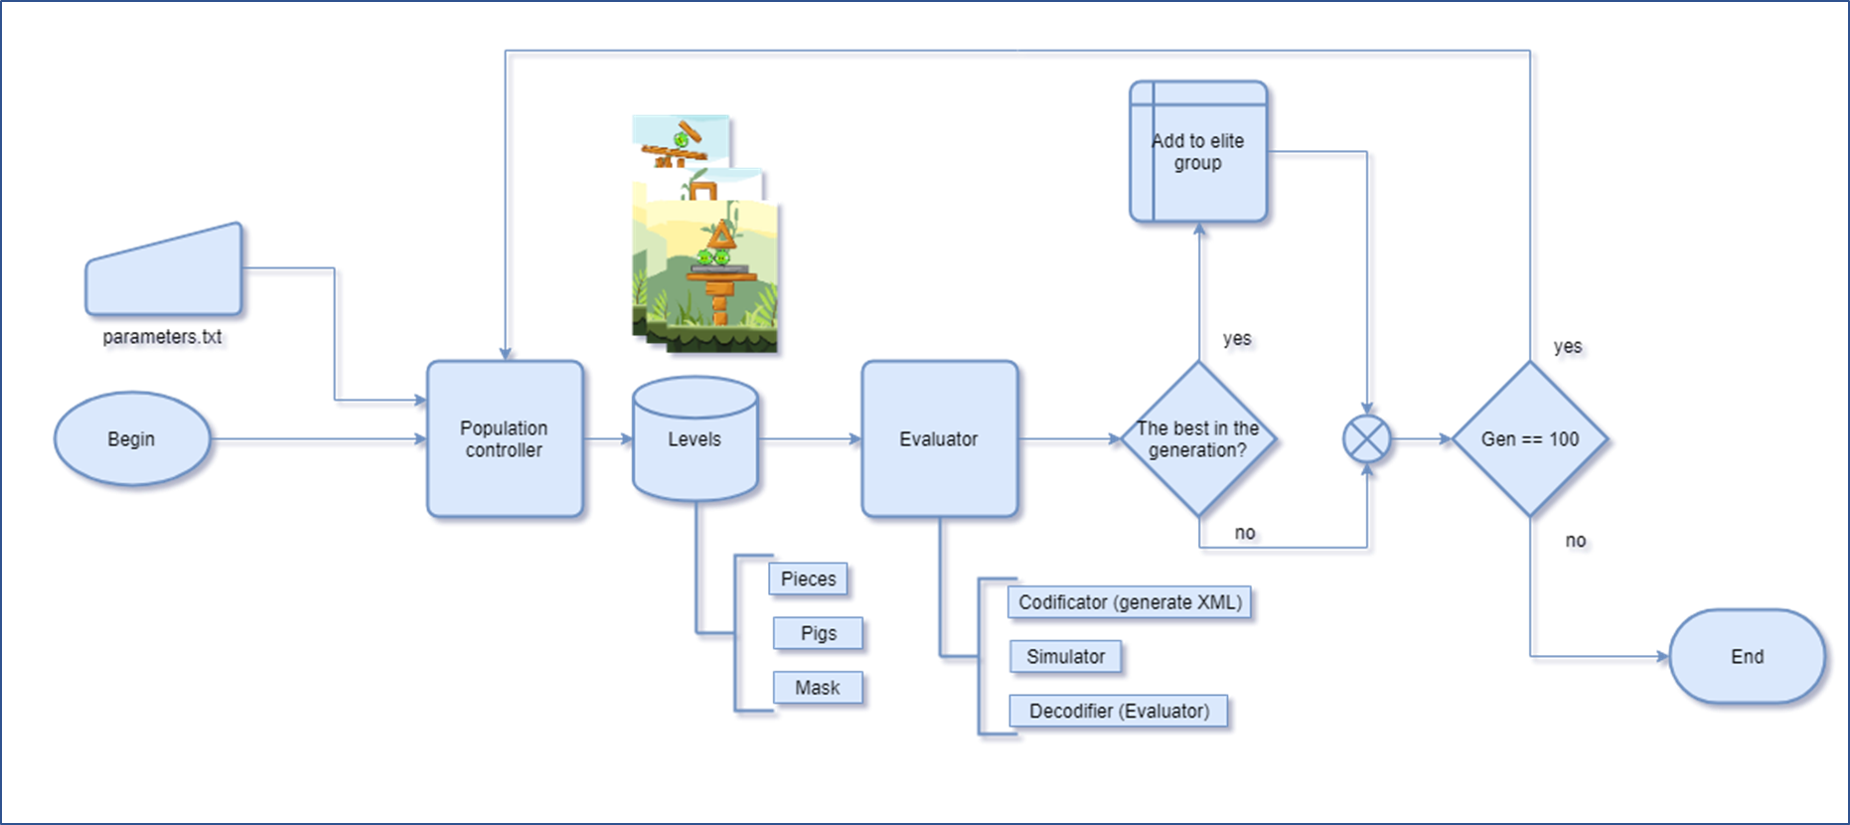
\includegraphics[width=160mm]{Images/new_model_v2.png}}
    \caption{New system diagram based on the parameter file and the new chromosome representation.}
    \label{new_model}
    \end{figure*}
    
    A diagram shows the main components and data flow of the proposed system
    is shown in Figure \ref{new_model} in which the parameter file of the competition 
    is integrated as an input. The layers of the system is explained next:
    
    \begin{itemize}
        \item Composite Generator:  This layer represents the composite blocks
        assigned to a particular individual as list of integer numbers, where
        each number represents a reference to a composite object including the
        ones generated by the OEE algorithm, the representation of this is was
        shown in figure \ref{old_chrom}.
        \item Structure layer: Individuals are represented by a list of seven
        integers, representing a mask in which integers assigned in each column
        represents the amount of composite blocks from the element layer that
        will be assigned to said column, a representation of this is shown on
        figure \ref{mask_layer}.
        \item Enemy layer: also known as pig layer, this layer is represented by
        two elements a single numeric value representing the total amount of
        pigs assigned to the level and an array of locations for the placement
        of these same pigs, a representation of it is shown on figure
        \ref{enemy_layer}. 
    \end{itemize}
    
    \begin{figure}[htbp]
        \centerline{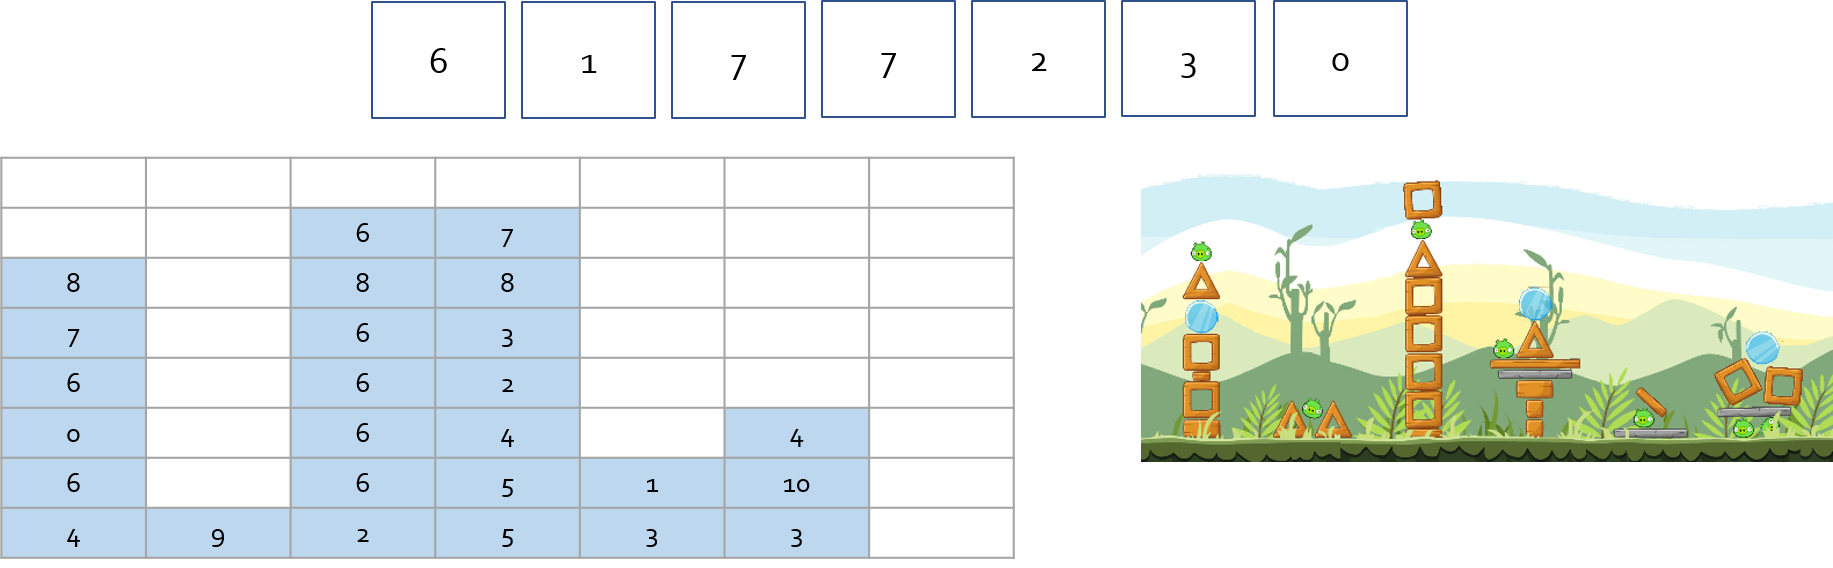
\includegraphics[width=80mm]{Images/mask_layer.png}}
        \caption{Mask array with column and phenotype representation.}
        \label{mask_layer}
    \end{figure}
    
    \begin{figure}[htbp]
        \centerline{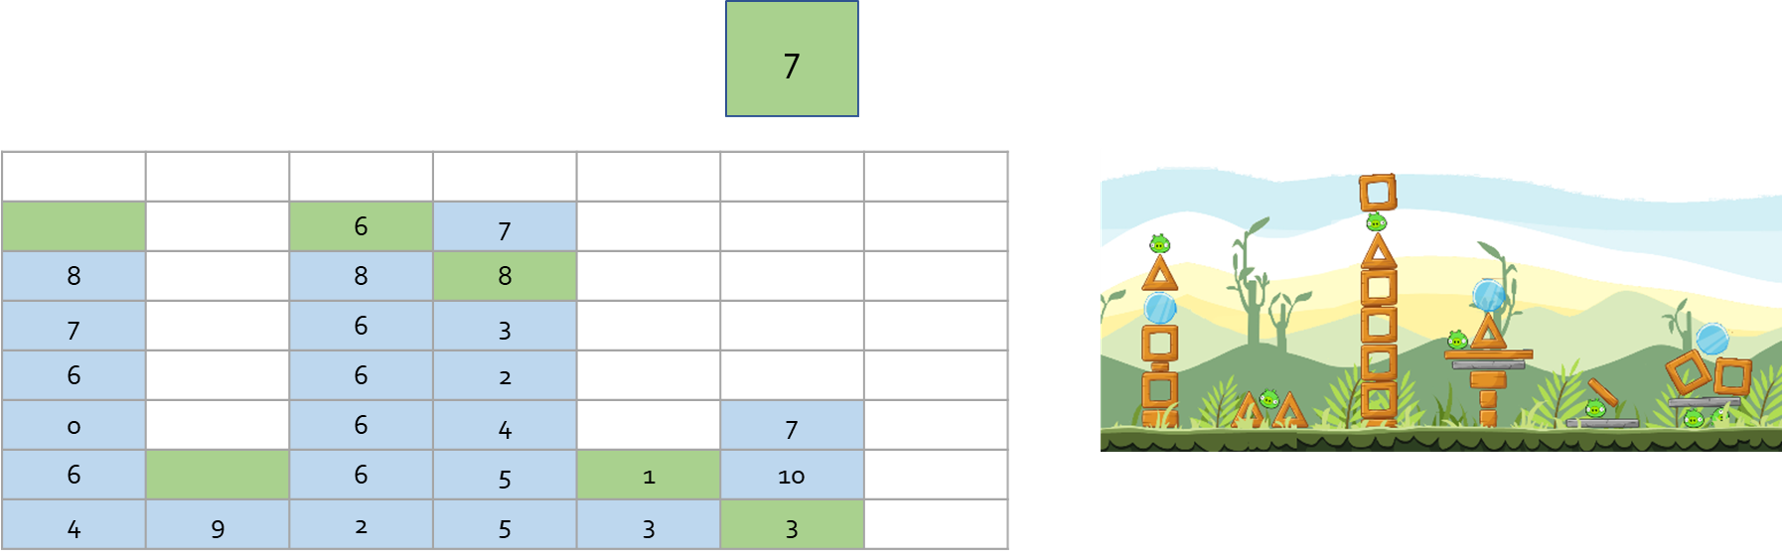
\includegraphics[width=80mm]{Images/enemy_layer.png}}
        \caption{Amount of pigs in a level, their location relative to the mask layer
         (green) and phenotype representation.}
        \label{enemy_layer}
    \end{figure}
    
    \subsection{Evolution of Levels} 

    Once structures are able to stand, there are other aspects we need to take
    in to account to evaluate their fitness. In this case we propose the use to
    reward both the \textit{"diversity"} and \textit{"uniqueness"} of a
    individual defining a fitness function considering:
    
    \begin{itemize}
        \item Hamming distance: a simple explanation for the \textit{Hamming
        distance} is that it is a calculation applied to a pair of strings where the
        objective is to find the minimum required number of substitutions required in
        order to convert a string exactly the same as the other, its formula is
        shown in equation \ref{hamming_distance}, since the formula itself locates
        the minimum number of substitutions then we compare the individual
        with the rest of the population trying to find the maximum number of
        substitutions required effectively using the formula to give a better fitness
        to those individuals that are different from the group.
        \item Shannon entropy: the Shannon entropy is used on information theory to
        calculate the disorder or uncertainty, in this case it will be used to
        determine if a level is \textit{"boring"} or \textit{"interesting"} based on
        the amount of entropy calculated according to the pieces used in a level
        where a low entropy is boring because if a determined level as a lot of
        repeated pieces then it will look simple, the formula used is shown in
        equation \ref{shannon_entropy} where the elements calculated are the pieces
        of a level and their appearance probability against all others.
    \end{itemize}
    
    \begin{equation}
        \begin{aligned}
        d = min \left\{ \ d(x,y): x,y \in C, if \: x \neq y, 1 \: else \: 0 \: \right\} \
        \end{aligned}
        \label{hamming_distance}
    \end{equation}
    
    \begin{equation}
        \begin{aligned}
        S = - \Sigma_i P_i \log P_i
        \end{aligned}
        \label{shannon_entropy}
    \end{equation}

    In order to select the parents of the next generation the parents are ordered by
    their fitness. There are two types of selection:
    
    \begin{itemize}
    % This needs more work.    
        \item Tournament selection: in order to select the parent by this method the
        system checks the amount of crossovers assigned, then calculates the amount
        of parent required to compete in pairs, then by doing a descendent selection
        the slots for the tournament are filled and the winners are calculated in
        each group.
        \item Roulette selection: this method of selection was first decided to be
        used directly by giving a proportional amount of chances to be selected
        according to the fitness of a individual, however since one of the
        objectives is to obtain variety of levels the roulette must first be ranked
        in order to ensure that low fitness individuals can be selected as parents.
    \end{itemize}
    
    As for the crossover operations the system currently uses two types, single
    point crossover and double point crossover, however this crossover operation is
    not only applied to the piece array of an individual, but it is also applied to
    the mask of said individual, this way the mask can ensure that some pieces of
    some children in the population are now placed in the level, this can bring the
    possibility that a mask that uses less pieces that it normally as can obtain a
    better fitness than one that uses all of them. An example of these two crossover
    types can be seen in figure \ref{crossover} in which the mask of an individual
    is combined with another and the resulting mask for the children have different
    amount of pieces to be placed.
    
    \begin{figure}[htbp]
        \centerline{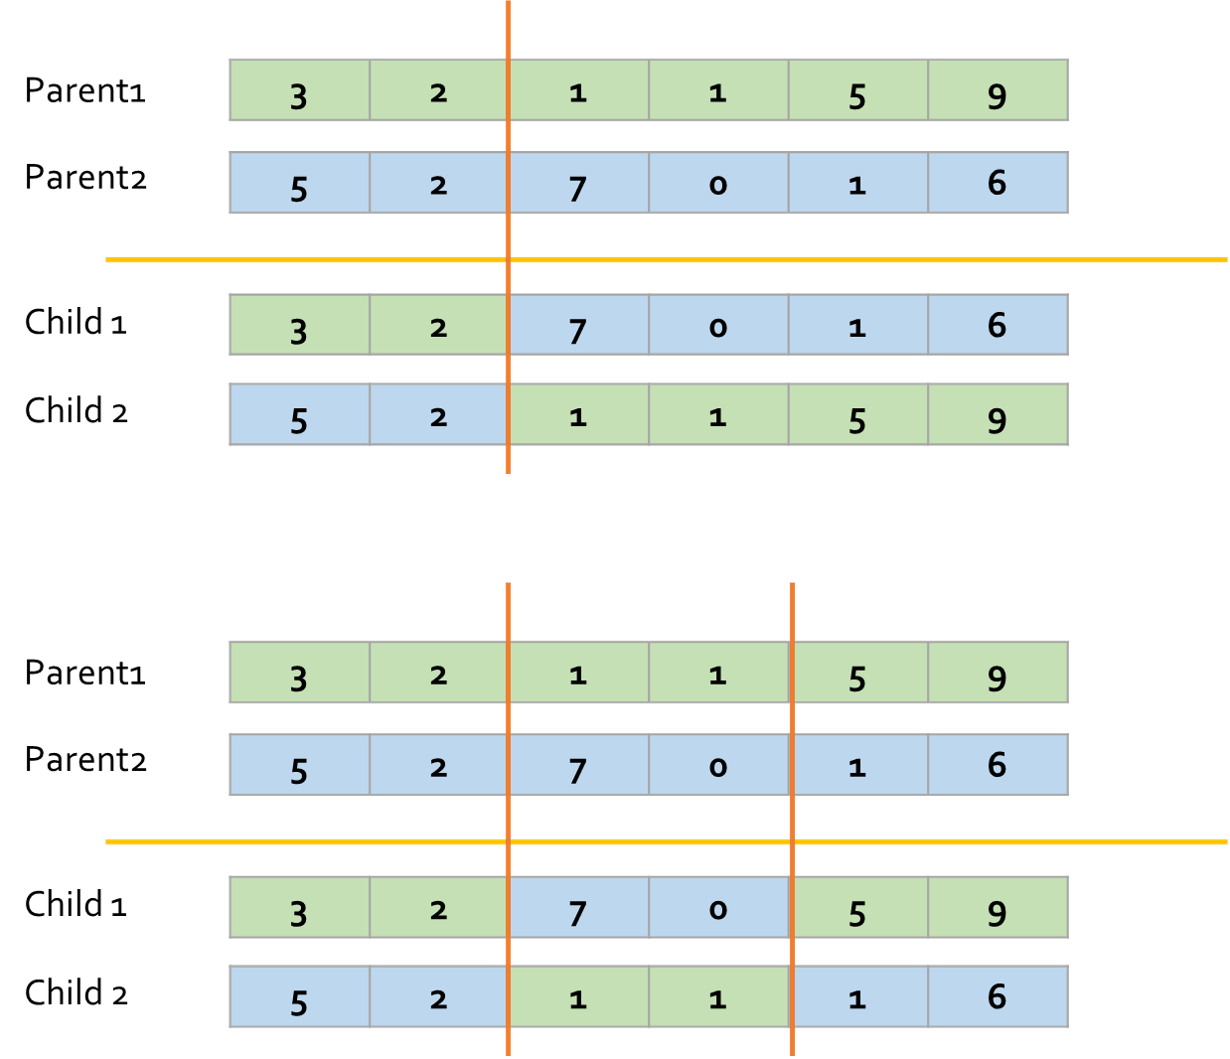
\includegraphics[width=80mm]{Images/crossover.png}}
        \caption{Single point crossover(up) and double point crossover(bottom) applied to an individual mask.}
        \label{crossover}
    \end{figure}
    
    The mutation operations of the generator work with the pieces layer of an
    individual, the four types of mutations are:
    
    \begin{itemize}
        \item Add or remove elements from the piece list
        \item Change the piece that is being used in a point of the list
        \item Change the material a piece is made offsets
        \item Change the x and y coordinates of a piece
    \end{itemize}
    
    These mutation operators do not have to be used all at the same time on a single
    individual but depending on the probabilities they can happen all at once,
    since most of the pieces on a individual are mostly the same type of
    material then at least the material mutation can occur on all or most of
    the individuals to ensure that all levels will not have all the pieces with
    the same material which could render a level \textit{"boring"} by the
    fitness function.
    

    
    Finally figure \ref{layer12_combine} and figure \ref{layer123_combine} represent 
    the way all the layers of an individual al combined to create a level after all 
    the selection, combination and mutation operations, first in figure \ref{layer12_combine}
    the composites layer is obtained from an individual, by a background process the 
    width and height of all composites are obtained, then using the mask from the same 
    individual the composites are placed in the order they are in their respective list 
    (left to right in the level) in case a mask is not able to accommodate all the 
    composites the remaining ones are not placed nor taken into account on the evaluation 
    process, in the opposite case that there are not enough composites to fill a mask 
    then the remaining areas are not taken into account as well, then in figure \ref{layer123_combine} 
    the previous combination of layers is evaluated by checking which placed composites 
    can hold a pig in the center or on the top of it, then the pigs are placed in the 
    same order the composites are placed (left to right) in the locations where one 
    is able to be placed.
    
    \begin{figure}[htbp]
        \centerline{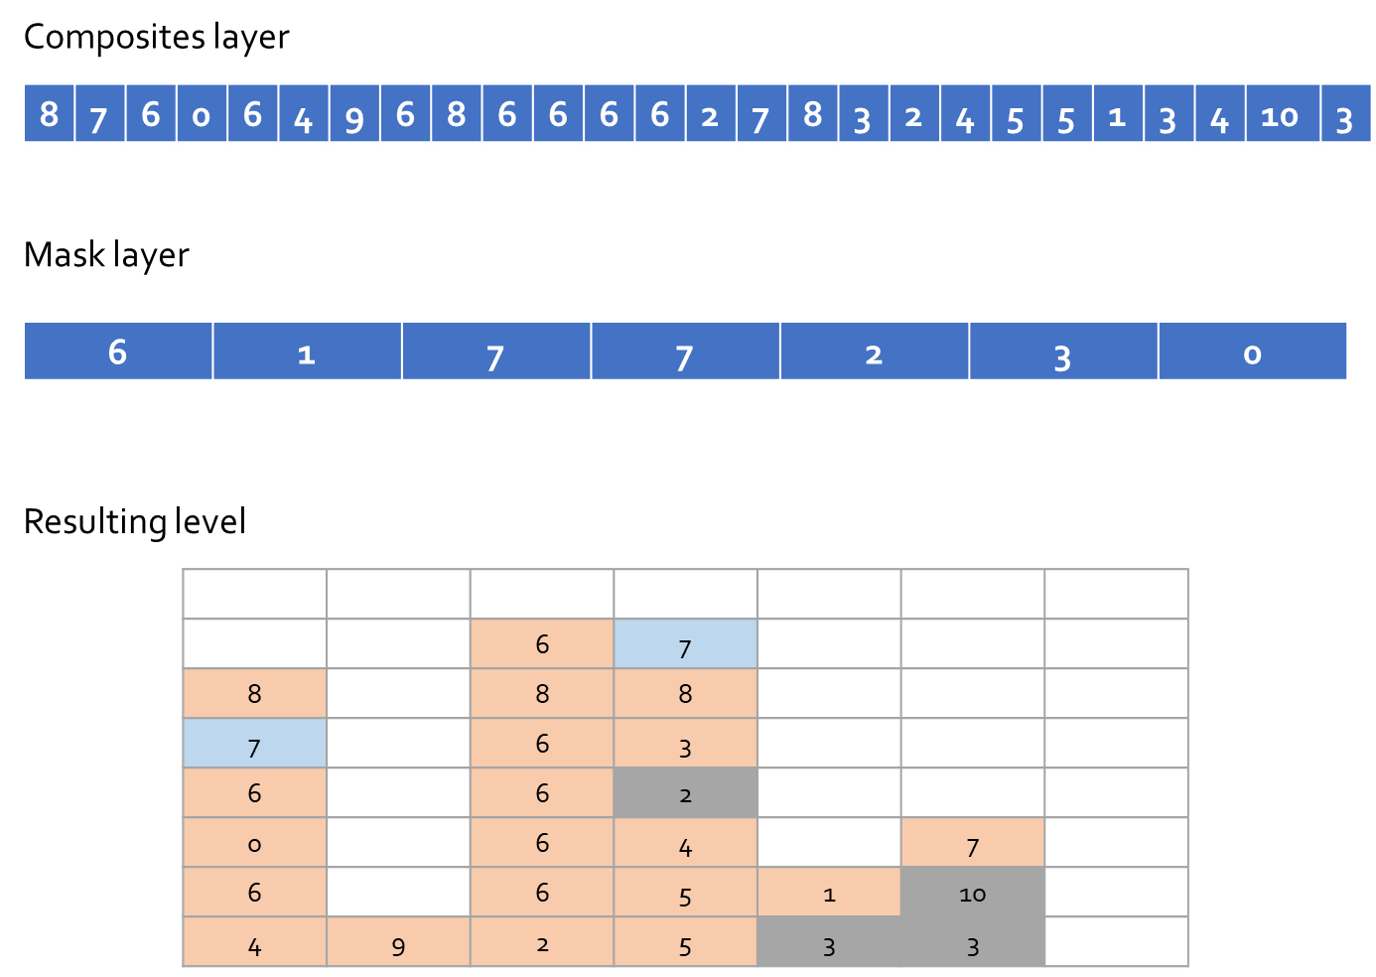
\includegraphics[width=80mm]{Images/layer12_combine.png}}
        \caption{Combination of composites layer and mask layer.}
        \label{layer12_combine}
    \end{figure}
    
    \begin{figure}[htbp]
        \centerline{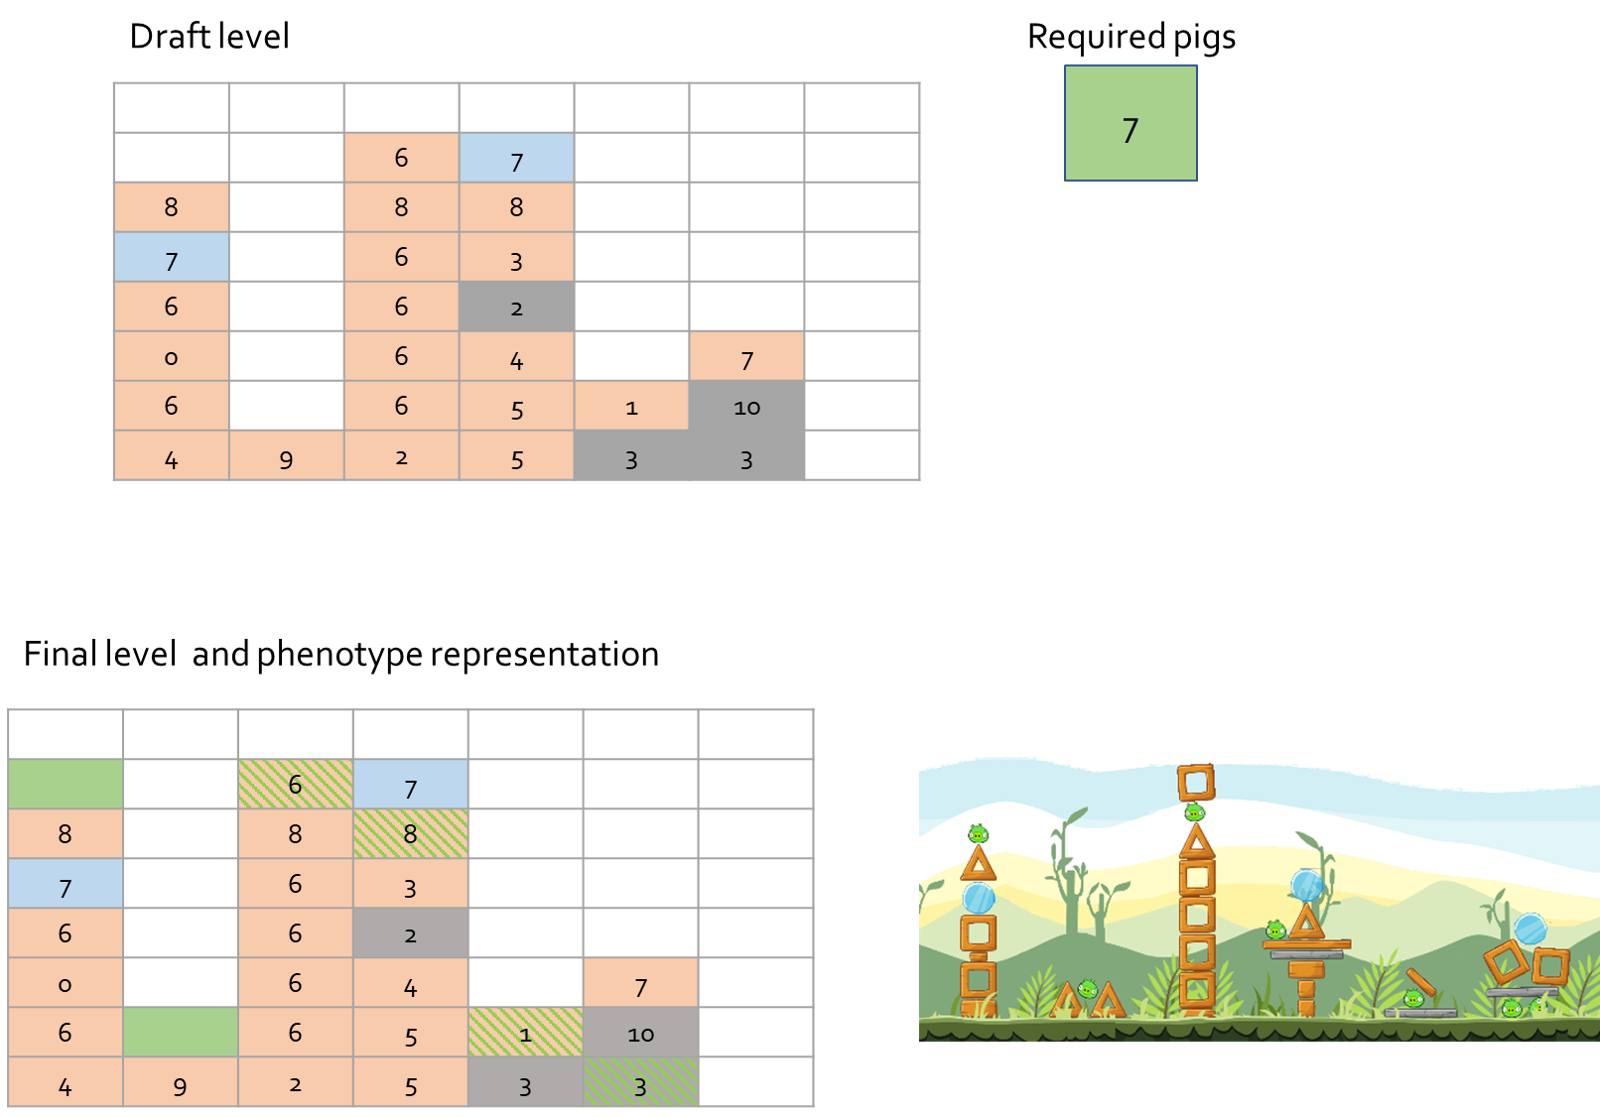
\includegraphics[width=80mm]{Images/layer123_combine.png}}
        \caption{Combination of figure \ref{layer12_combine} layers with pig layer.}
        \label{layer123_combine}
    \end{figure}
    
    Using all these configurations the system is capable of creating levels, some of
    them playable as shown in figure \ref{result_1} however the levels that can be
    generated are far from optimized to be played on, this is an issue that must be
    changed in future instances but the generator itself is able to be used as a
    base for a more complex one, and as shown in the future work section these issues
    can be solved by different means.
    
    \begin{figure*}[htbp]
        \centerline{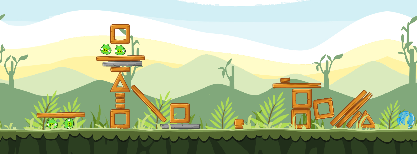
\includegraphics[width=160mm]{Images/Result_n2.png}}
        \caption{Example of resulting level with current system.}
        \label{result_1}
    \end{figure*}
    
    \section{Conclusions and future work}
    \label{conclusion}
    
     The system has been able to generate levels that fulfill the requirements
     provided by the parameters file, however a way to evaluate that the levels
     generated are indeed \textit{"fun"} or \textit{"interesting"} is still
     needed, at this point we could evaluate the levels by applying an approach
     used in previous competitions:
     \begin{itemize}
        \item User survey, in case a survey is used as an evaluation tool then first
        the system has to generate the levels and a group of people must participate
        by playing the levels and answering a set of questions afterwards, the
        questions themselves must try to capture the feeling of a person towards the
        game like questioning if a level was too easy or too difficult to solve, if
        the generated structures look interesting or if the level required them to
        strategize how to use the provided birds to solve the level, the survey must
        be applied to a equal quantity of people of three different game skill
        levels,\textit{"non video game players"}, \textit{"casual video game
        players"} and \textit{"avid video game players"}, this way we can evaluate a
        level or the entire system by knowing if all skill levels did not enjoyed a
        level because it was too simple or easy.
        \item By using a naive agent, if a naive agent is used to play the levels we
        can obtain data of how the agent solves the levels placed before them, and
        the way to evaluate if the level is or not \textit{"interesting"} will be by
        checking how easily the agent is able to solve a level, the point here is
        to have a level that cannot be solved by a single movement but to have one
        that a human player has to think a while to solve trying to place the
        difficulty of a level just at the middle point between easy and hard
        difficulty levels.
    \end{itemize}
        
    Other aspects that the system need to improve is in the processing time
    required, since the current way to calculate the fitness and create the next
    generations of a population requires the system to execute
    simulations of the levels on every generation that passes, therefore increasing
    the time it takes to complete an entire cycle of execution. In order to
    change this we require to create a way to evaluate a level using only the
    information of the pieces, locations and pigs locations and using this data to
    predict the way a level will behave when placed in a real simulation environment
    therefore drastically reducing execution times. %You can also take into account restrictions without simulation, as we do in our paper, or use a Physics engine - JJ

    We were able to fulfill our objective of generating levels that could be played;
    however, as seen in our figures, the current state of this system is still in the development 
    phase, and some modifications must be applied in order to optimize some aspects of it. For instance  
    by using a different way of generating individual we were able to reduce the process 
    time required on a full system execution; however we need to search for a way to 
    avoid using the software to evaluate the individuals, this way we expect to reduce 
    drastically the time required to process the data of the levels.  % Cite our paper, where we do exactly that - JJ
    
    Finally a different method to evaluate the individuals must be created. Since the current evaluation method allows us to generate playable levels,  
    these levels are far from ideal in the way that they only use a certain range of
    items present in the game therefore reducing the potential of a level, we expect
    to make the current fitness function work the most efficient that it can but
    another possible solution is found a good combination of formulas to generate
    the fitness function.

\section*{Acknowledgments}

This work has been supported in part by: Ministerio espa\~{n}ol de
Econom\'{\i}a y Competitividad under project TIN2017-85727-C4-2-P (UGR-DeepBio).


\bibliographystyle{IEEEtran}
\bibliography{References/article_references.bib}

\end{document}
